\subsection{Queue Manager}\label{comp:queueManager}
\begin{figure}[H]
	\centering
	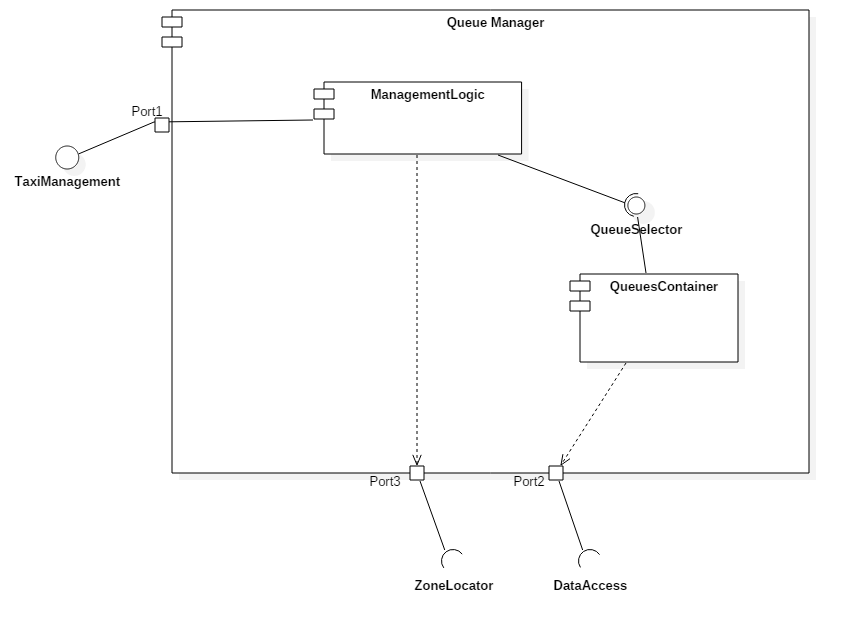
\includegraphics[scale=0.5]{../"Analysis Documents"/components/queueManager}
	\label{fig:queuemanager}
	\caption{Queue Manager internal structure}
\end{figure}
\subsubsection{Provided interfaces}
\begin{table}[H]
	\begin{longtable}{| p{0.3\textwidth} | p{0.3\textwidth} | p{0.4\textwidth} |}
		\hline
		\textbf{Provided Interface} & \textbf{Dedicated user} & \textbf{Description} \\ \hline
		TaxiManagement & Taxi Manager component & Provides the methods for adding, removing and retrieving taxi drivers to the data structure (queue) \\ \hline
	\end{longtable}
	\caption{Queue Manager: provided interfaces}
	\label{tab:queuemanager:providedInterfaces}
\end{table}
\subsubsection{Required interfaces}
\begin{table}[H]
	\begin{longtable}{| l | p{.80\textwidth} |}
		\hline
		\textbf{Required Interface} & \textbf{Description and usage} \\ \hline
		Zone Locator & Gets the list of the zones at the start up of the system in order to create the needed queues \\ \hline
		Data Access & Maintains the queues in the database \\ \hline
	\end{longtable}
	\caption{Queue Manager: required interfaces}
	\label{tab:queuemanager:requiredInterfaces}
\end{table}
